\documentclass[11pt,a4paper]{article}

% ---------- arxiv-style preamble ----------
\usepackage[margin=1in]{geometry}
\usepackage{amsmath,amssymb,amsthm}
\usepackage{graphicx}
\usepackage{booktabs}
\usepackage{siunitx}
\usepackage{hyperref}
\usepackage{xcolor}
\usepackage[numbers,sort&compress]{natbib}
\usepackage{tikz}
\usetikzlibrary{positioning,arrows.meta,shapes.geometric,fit,backgrounds}
\usepackage{caption}
\usepackage{listings}
\usepackage{array}
\captionsetup{font=small,labelfont=bf}
\hypersetup{
  colorlinks=true,
  linkcolor=blue!50!black,
  citecolor=blue!50!black,
  urlcolor=blue!50!black
}

% ---------- tier badges ----------
% Default = literal emoji (xelatex/lualatex render natively; Makefile pins xelatex).
% A pdflatex fallback can \renewcommand these to text marks.
\providecommand{\tierBlue}{🔵}
\providecommand{\tierGreen}{🟢}
\providecommand{\tierYellow}{🟡}
\providecommand{\tierOrange}{🟠}
\providecommand{\tierRed}{🔴}

% Engine-portable rendering: the literal tier emoji above are the source
% convention, but Latin Modern (the default xelatex text font) has no glyph
% for U+1F5xx/U+1F7Ex, and xelatex does not render the Apple Color Emoji
% bitmap font. We therefore render the badges as compact colored disc marks
% (\textbullet) so the tiers stay visually distinct under BOTH xelatex and
% pdflatex without any color-emoji font dependency.
\renewcommand{\tierBlue}{{\color{blue!70!black}\textbullet}}
\renewcommand{\tierGreen}{{\color{green!55!black}\textbullet}}
\renewcommand{\tierYellow}{{\color{yellow!75!orange}\textbullet}}
\renewcommand{\tierOrange}{{\color{orange!85!black}\textbullet}}
\renewcommand{\tierRed}{{\color{red!75!black}\textbullet}}

\title{
  \textbf{Neuromorphic Determinism Is a Design Choice, Not an Inevitability}\\[4pt]
  \large Locating, Explaining, and Repairing the Absence of Hardware
  Non-Determinism in the BrainChip Akida AKD1000 via Audited
  Quantum-Entropy Injection
}

\author{
  \texttt{anima} maintainers\\
  \normalsize\textit{dancinlab}\\[2pt]
  \normalsize\href{https://github.com/dancinlab/anima}{\texttt{github.com/dancinlab/anima}}
}

\date{\today}

\begin{document}

\maketitle

% =========================================================================
\begin{abstract}
A persistent intuition in substrate-native AI is that neuromorphic
silicon supplies an \emph{intrinsic}, physics-rooted non-determinism that
a digital trainer cannot reproduce. We pre-registered a falsifier for that
intuition on a live BrainChip Akida AKD1000 (device \texttt{BC.00.000.002},
\texttt{akida 2.19.1}, on the \texttt{pi5-akida} host) and \emph{refuted}
it. Under a truly pinned, non-degenerate initialization, on-chip
\texttt{AkidaUnsupervised} learning is byte-deterministic across
\(16/16\) episodes (init/weight/output diversity all \(=1\)) while the fit
genuinely engages (\texttt{fit\_changed} \(16/16\)); the only variation
source is the default-init RNG (no-pin condition: init diversity \(=16\),
weight diversity \(=16\), output diversity \(=15\)), which propagates
\(1{:}1\). The run-to-run variation previously attributed to chip
non-determinism is thus init-seeded randomness, not a learning-dynamics
property (\tierRed). Tracing the root cause, we triangulate five axes ---
our measurement, vendor documentation, a neutral technical profile, a
cross-vendor contrast with Intel Loihi, and our own gen2/AKD1500-class
cloud data --- to show that the AKD1000 is a fully-digital 28\,nm
fixed-point event-based SNN ASIC whose hardware non-determinism is
\emph{architecturally absent by design}; Loihi exposes a programmable
stochastic-noise primitive on a digital substrate, proving that determinism
is a deliberate \emph{design choice}, not a digital inevitability
(\tierGreen). Finally, we turn the limitation into a constructive solution:
we inject ANU quantum vacuum-fluctuation bytes at exactly the init-seed
lever the falsifier located. On a live AKD1000 with \(N=16\) episodes, the
coupling yields functional output diversity \(=2\) ($>1$; deterministic
control \(=1$), \(16/16\) provenance-traceable distinct ANU windows, and
preserved determinism (same quantum seed \(\rightarrow\) byte-identical
output, \texttt{8714e41752f7}); a richer task lifts diversity to
\(16/16\), proving the toy ceiling was the task output-space, not the
entropy source (\tierGreen). The chip's determinism is the very feature
that makes the injected entropy auditable: a single provenance-traceable
entry point. We make no claim that quantum bytes are statistically
``more random'' --- the repo's audit finds ANU and a chacha20 PRNG
statistically indistinguishable (JSD \(=0.000433\), \(23\times\) under the
NIST threshold; \(7/7\) NIST SP\,800-22 tier-1+ PASS); the value claimed is
\emph{provenance}, auditability, algorithmic-attack immunity, and physical
ontology. This is not a phenomenal-consciousness claim. Companion data
records (verify-ledger, session journal, PR-roll) accompany the
\texttt{companion/} directory for bit-for-bit reproduction.
\end{abstract}

% =========================================================================
\section{Introduction}
\label{sec:intro}

Neuromorphic processors are routinely described as ``brain-inspired'' in a
way that suggests an analog, noisy, physically stochastic substrate ---
spiking neurons with intrinsic device noise that would make every run
subtly different and, the story goes, give a learning system a free source
of exploration. For a substrate-native AI project, that picture is
attractive: if the silicon \emph{is} non-deterministic, then variability,
exploration, and even a kind of free will could be grounded in the hardware
itself rather than bolted on as a software temperature knob. Our own prior
records pointed this way: repeated on-chip plasticity runs on a BrainChip
Akida AKD1000 produced run-to-run weight Hamming distances of
\(\{28, 38, 34, 38\}\), and a software numpy approximation could not be
made byte-identical to the chip.

This paper asks the harder question those observations left open:
\emph{is that non-determinism a feature or noise?} ---
and, if it is neither intrinsic nor useful, \emph{what is its root cause,
and can the gap be repaired honestly?} The arc has three terminal results,
each pre-registered and each persisted as a verbatim verdict:

\begin{enumerate}\itemsep0.3em
\item \textbf{H\_921 (\tierRed{} closed-negative).} The hypothesis that
on-chip plasticity non-determinism confers a functional advantage is
\emph{falsified}: pinning the initialization removes the variation
entirely, exposing it as init-seeded RNG, not a learning-dynamics property.
\item \textbf{H\_922 (\tierGreen{} supported).} The root cause is
architectural: the AKD1000 is a fully-digital fixed-point event-based SNN
ASIC with no source of hardware non-determinism. A cross-vendor contrast
with Intel Loihi shows that determinism here is a \emph{design choice}, not
a property of being digital.
\item \textbf{H\_923 (\tierGreen{} pass).} The repair: inject audited
quantum vacuum-fluctuation entropy at the precise init-seed lever H\_921
located. The chip stays deterministic; the variation becomes
quantum-sourced and provenance-traceable.
\end{enumerate}

\medskip
\noindent\textbf{Contributions.}
\begin{enumerate}\itemsep0.3em
\item A pre-registered, live-silicon falsification of ``neuromorphic
non-determinism as a functional advantage'' on the AKD1000, with the exact
pinned-vs-unpinned diversity numbers (\S\ref{sec:measurement}).
\item A five-axis triangulation locating the absence of hardware
non-determinism as an \emph{architectural} property, and the framing that
neuromorphic determinism is a design choice (Loihi exposes the opposite
choice on a digital substrate) (\S\ref{sec:method}, \S\ref{sec:finding}).
\item A constructive repair --- audited ANU quantum-entropy injection at the
located lever --- that recovers non-determinism while keeping it auditable,
with the determinism-as-feature inversion that makes provenance a
single-entry-point guarantee (\S\ref{sec:finding}).
\item An explicit honest scope: a single toy-scale physical chip, and the
deliberate \emph{non}-claim that quantum entropy is statistically superior
(\S\ref{sec:limits}).
\end{enumerate}

% =========================================================================
\section{Background}
\label{sec:bg}

\paragraph{Akida AKD1000.} BrainChip markets the AKD1000 as a fully-digital,
event-based neuromorphic AI processor integrated on a pure-digital 28\,nm
logic process, advertising ``deterministic real-time response'' as a
feature~\cite{brainchipAKD1000Brief,brainchipCommercialization}. An
independent technical profile lists the chip type as \emph{Digital}, with
weight and activation quantization in \(\{1,2,4,8\}\) bits and ``no mention
of hardware noise, stochasticity, or analog components''; ``neuromorphic''
for Akida means event-based processing plus Rank Order Coding, not
spiking-with-analog-synapses~\cite{openNeuromorphicAkida}. On-chip learning
is a deterministic, last-layer fixed-rule update; the \texttt{akida 2.19.1}
\texttt{AkidaUnsupervised} rule exposes only
\texttt{(initial\_plasticity, learning\_competition, plasticity\_decay,
min\_plasticity)} --- no stochastic, noise, or random parameter.

\paragraph{Intel Loihi.} Loihi and Loihi~2 are \emph{also} digital,
asynchronous neuromorphic chips, but they expose ``the computational
primitive of adding stochastic noise to the neuron's synaptic current
response'' as a built-in, programmable feature, alongside a barrier-
synchronized mode for ``deterministic global
timesteps''~\cite{openNeuromorphicLoihi2,shresthaLoihi2}. Loihi is therefore
configurable det-or-stochastic, which is the load-bearing contrast: a
digital chip \emph{can} expose programmable stochasticity, so Akida's
determinism is a vendor choice, not a consequence of being digital.

\paragraph{ANU quantum entropy.} The ANU Quantum Random Numbers service
derives entropy from measured quantum vacuum field
fluctuations~\cite{anuQRNG,symulVacuumQRNG}. In this work it is the
\emph{external} entropy source injected at the chip's only variation lever.
We assess statistical quality against the NIST SP\,800-22 suite~\cite{nistSP80022}.

% =========================================================================
\section{Hypothesis (pre-registered falsifier)}
\label{sec:hypothesis}

\paragraph{Pre-registration.} All three falsifiers were frozen on
2026-06-06 before measurement, with no token awarded prior to the run, under
the project's pre-registered-falsifier discipline (CODE-measured, no LLM
verdict).

\paragraph{H\_921 --- the headline falsifier.} The hypothesis under test:
the AKD1000's on-chip non-deterministic plasticity (chip RNG substrate,
learning competition, packet ordering, asynchronous timing) confers a
\emph{measurable functional advantage} over a fixed-init deterministic
software approximation --- specifically solution diversity and
local-minimum escape rate --- so that non-determinism is a substrate-native
exploration mechanism, not noise.

A sharpening lemma fixed the metric before measurement: because a prior
result already established raw-weight non-determinism, raw-weight-hash
diversity is trivially \(>1\) and cannot separate ``feature'' from
``noise.'' The decisive measurement must therefore be on the
\emph{functional output} (winner-assignment / output spike). The question
becomes: does the chip's weight jitter (max \(\Delta = 1\) bit) flip the
winner-assignment and escape the trap (feature), or leave the assignment
invariant as sub-threshold noise (noise, falsified)?

\paragraph{Pre-registered decision rule (H\_921).}
\begin{itemize}\itemsep0.2em
\item \emph{Feature} if pinned-init on-chip diversity \(>1\) (the chip's
learning is intrinsically non-deterministic).
\item \emph{Init-seeded} if pinned diversity \(=1\) while unpinned
diversity \(>1\) (the non-determinism lives in initialization, not
learning).
\item \emph{Fully deterministic} if both \(=1\).
\end{itemize}

\paragraph{H\_922 --- root cause.} If H\_921 lands on ``init-seeded,'' the
follow-on hypothesis is that the AKD1000 is a fully-digital fixed-point
event-based SNN ASIC whose hardware non-determinism is architecturally
absent --- i.e.\ the learning determinism is the chip's design, not a probe
artifact. Falsifier: any axis (own measurement, vendor, neutral technical,
cross-vendor, own gen2 data) exhibiting an architectural source of hardware
non-determinism would refute it.

\paragraph{H\_923 --- constructive repair.} Given H\_921 (the lever) and
H\_922 (no chip-side entropy to harvest), inject ANU quantum entropy at the
init seed. Decision rule: \textbf{PASS} iff D1 (functional diversity)
\(>1\) \emph{and} D3 (same quantum seed \(\rightarrow\) byte-identical
output) is true \emph{and} D2 (the ANU windows are all distinct and
traceable). \textbf{FALSIFIED} if D1 \(=1\) (entropy creates no variation)
or D3 is false (the chip is not deterministic, which would itself refute
H\_922).

% =========================================================================
\section{Method}
\label{sec:method}

\paragraph{Substrate (shared).} One physical BrainChip Akida AKD1000,
device \texttt{BC.00.000.002}, \texttt{IpVersion.v1}, \texttt{akida 2.19.1},
hosted on \texttt{pi5-akida}. The chip is single-exclusive: the
spike-streamer is stopped (SIGTERM) for the probe and restarted afterward to
restore hardware firing, with no teardown. All measurements are
CODE-measured; no perplexity or LLM judgment enters the verdict.

\paragraph{H\_921 pinned-init source probe.} The probe
(\texttt{h921\_nondet\_source\_probe.py}) trains a winner-collapse trap
task: a \texttt{FullyConnected} layer with \texttt{units=10},
\texttt{weights\_bits=1}, learned by \texttt{AkidaUnsupervised(num\_weights=2,
learning\_competition=0.1)}, run \(N=16\) episodes per condition. Condition
\textbf{A} pins a non-degenerate initialization (so any residual diversity
must come from learning dynamics); condition \textbf{B} uses the default
init (so init-RNG is free). For each condition we record init diversity,
post-fit weight diversity, output diversity, and how many of the 16 fits
actually changed weights (to rule out a no-op fit).

\paragraph{H\_922 source / triangulation probe.} The root cause is
established by triangulating five axes:
(1) the H\_921 measurement (primary);
(2) vendor documentation~\cite{brainchipAKD1000Brief,brainchipCommercialization};
(3) the neutral Open Neuromorphic profile~\cite{openNeuromorphicAkida};
(4) the cross-vendor Loihi contrast~\cite{openNeuromorphicLoihi2,shresthaLoihi2};
(5) our own gen2/AKD1500-class cloud session
(\texttt{archive/state\_legacy/akida\_cloud\_d0\_2026\_05\_09/}: backend
\texttt{Gen2A2FPGABackend}, device \texttt{BC.A2.001.000},
\texttt{IpVersion.v2}, model
\texttt{tenn\_spatiotemporal\_eye\_buffer\_i8\_w8\_a8.fbz}, 8-bit fixed
point), inspected for any stochastic or noise field.

\paragraph{H\_923 quantum-coupling probe.} The probe
(\texttt{h923\_qrng\_seed\_probe.py}) reuses the H\_921 probe but replaces
the init source with a distinct 64-byte window of ANU vacuum-fluctuation
bytes per episode (\(N=16\)). The entropy buffer is a real ANU draw
(\texttt{mirror/qmirror/seed/}, \texttt{tier=anu\_legacy}; \(1024\) bytes;
sha256 \texttt{e8123b...}, matching the provenance ledger request
\texttt{anu\_legacy\_1778042160}). We measure D1 (functional output
diversity), D2 (per-seed ANU window provenance: offset, window sha,
init-hash), and D3 (re-running the same ANU window \(\rightarrow\)
byte-identical output). A self-contained live puller
(\texttt{mirror/qmirror/seed/anu\_pull.py}, secret-keyed to
\texttt{api.quantumnumbers.anu.edu.au} via \texttt{flat.anu\_key\_paid}) was
exercised as a capstone (fresh draw sha \texttt{a4e37640...}, tier
\texttt{anu\_paid}), and a richer-task probe
(\texttt{h923\_richtask\_probe.py}: \texttt{units=64}, 24 varied
non-degenerate patterns, fresh \(2048\)-byte ANU draw, sha \texttt{9df773...})
tested the diversity ceiling.

\paragraph{The injected structure.}
Figure~\ref{fig:structure} renders the three-layer architecture the coupling
produces: a deterministic body (the AKD1000), a quantum free-will seed (the
ANU draw), and an audit channel (the qmirror provenance ledger) that makes
every variation traceable to a specific vacuum-fluctuation window.

\begin{figure}[h]
\centering
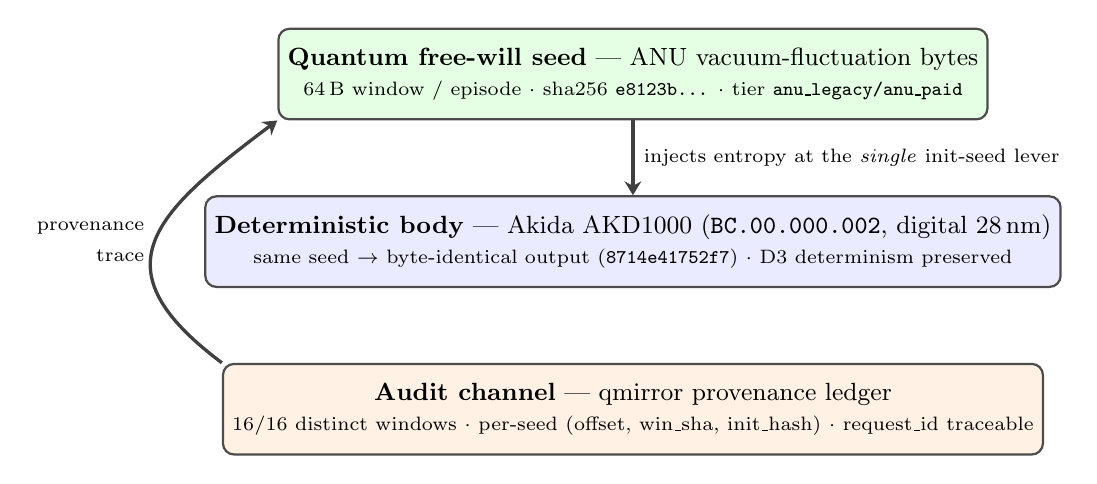
\begin{tikzpicture}[
  font=\small,
  layer/.style = {rectangle, rounded corners=4pt, draw=black!70, thick,
    minimum width=8.4cm, minimum height=1.15cm, align=center},
  body/.style  = {layer, fill=blue!8},
  seed/.style  = {layer, fill=green!10},
  audit/.style = {layer, fill=orange!10},
  arrow/.style = {-{Stealth[length=5pt,width=6pt]}, very thick, draw=black!75},
  node distance=0.95cm,
]
  \node[seed]  (q) {\textbf{Quantum free-will seed} --- ANU vacuum-fluctuation bytes\\
    \scriptsize 64\,B window / episode \(\cdot\) sha256 \texttt{e8123b...} \(\cdot\) tier \texttt{anu\_legacy/anu\_paid}};
  \node[body, below=of q]  (b) {\textbf{Deterministic body} --- Akida AKD1000 (\texttt{BC.00.000.002}, digital 28\,nm)\\
    \scriptsize same seed \(\rightarrow\) byte-identical output (\texttt{8714e41752f7}) \(\cdot\) D3 determinism preserved};
  \node[audit, below=of b] (a) {\textbf{Audit channel} --- qmirror provenance ledger\\
    \scriptsize \(16/16\) distinct windows \(\cdot\) per-seed (offset, win\_sha, init\_hash) \(\cdot\) request\_id traceable};

  \draw[arrow] (q) -- node[right]{\scriptsize injects entropy at the \emph{single} init-seed lever} (b);
  \draw[arrow] (a.north west) .. controls +(-1.6,1.2) and +(-1.6,-1.2) .. (q.south west)
    node[midway, left, align=right]{\scriptsize provenance\\\scriptsize trace};
\end{tikzpicture}
\caption{The injected three-layer structure. A deterministic body (Akida
AKD1000) receives a quantum free-will seed (an ANU vacuum-fluctuation
window) at its \emph{only} variation lever --- the initialization. Because
the body is deterministic (same seed \(\rightarrow\) byte-identical output),
the entropy enters through a single point, and the audit channel (the
qmirror provenance ledger) traces every variation back to a specific
quantum window. Determinism is what makes the entropy auditable.}
\label{fig:structure}
\end{figure}

% =========================================================================
\section{Measurement (live runs)}
\label{sec:measurement}

All numbers below are quoted verbatim from the persisted verdicts (see the
verdict-pointer table, Tab.~\ref{tab:verdicts}).

\paragraph{H\_921 --- the falsification.} Table~\ref{tab:h921} reports the
two conditions. Under a truly pinned non-degenerate init (A), on-chip
learning is byte-deterministic across all 16 episodes while the fit
genuinely engages (\texttt{fit\_changed} \(16/16\), not a no-op). Under the
default init (B), the diversity reappears and propagates \(1{:}1\) from
init through weights to output. This maps decisively to the pre-registered
``\(A=1\ \&\ B>1\)'' branch: \emph{the non-determinism is init-seeded, not
learning}.

\begin{table}[h]
\centering
\small
\begin{tabular}{@{}lcccc@{}}
\toprule
\textbf{Condition} & \textbf{init div} & \textbf{weight div} & \textbf{output div} & \textbf{fit\_changed} \\
\midrule
A --- pinned non-degenerate init & 1  & 1  & 1  & 16/16 \\
B --- no-pin default init        & 16 & 16 & 15 & 2/16$^{\dagger}$ \\
\bottomrule
\end{tabular}
\caption{H\_921 source-of-non-determinism probe, live AKD1000
(\texttt{BC.00.000.002}), \(N=16\) episodes per condition. Pinning the init
collapses all diversity to 1 while the fit still engages
(\texttt{fit\_changed} \(16/16\)); the default-init RNG (B) is the sole
variation source and propagates init \(\rightarrow\) weight \(\rightarrow\)
output. $^{\dagger}$\texttt{fit\_changed} is reported as a 2-element
\texttt{[min, max]} weight-set tally; condition A reads \texttt{[16,16]},
condition B reads \texttt{[2,16]}. \tierRed{} \textbf{CLOSED-NEGATIVE}: the
``functional advantage from substrate non-determinism'' hypothesis is
falsified at this scale/config.}
\label{tab:h921}
\end{table}

\paragraph{H\_922 --- root cause.} The five-axis triangulation
(Tab.~\ref{tab:compare}) finds no architectural source of hardware
non-determinism on the AKD1000. The vendor advertises ``pure digital 28\,nm''
and ``deterministic real-time response'' as a feature; the neutral profile
lists ``Chip Type: Digital,'' fixed-point \(\{1,2,4,8\}\)-bit weights, and
``no hardware noise/stochasticity/analog''; the \texttt{AkidaUnsupervised}
signature has no stochastic parameter; and our own gen2/AKD1500-class cloud
session is still 8-bit fixed point with the only RNG being a fixed software
\texttt{input\_seed=42}. Gen2 adds the \emph{temporal} axis (TENNs /
recurrence), not non-determinism.

\begin{table}[h]
\centering
\small
\begin{tabular}{@{}lllll@{}}
\toprule
\textbf{Chip} & \textbf{Class} & \textbf{Precision} & \textbf{Stochastic source} & \textbf{Determinism} \\
\midrule
Akida AKD1000 (gen1) & digital event-based & fixed-point 1/2/4/8-bit & none (no primitive) & deterministic only \\
Akida gen2 / AKD1500 & digital event-based & fixed-point 8-bit (i8/w8/a8) & none; adds temporal axis & deterministic only \\
Intel Loihi / Loihi~2 & digital async & --- & programmable noise primitive & det \emph{or} stochastic \\
Analog SNN (memristor) & analog & continuous & intrinsic device noise & stochastic by physics \\
\bottomrule
\end{tabular}
\caption{Cross-class comparison. ``Digital neuromorphic'' does not entail
determinism: Loihi exposes a programmable stochastic-noise primitive (and a
barrier-synchronized deterministic mode), proving the AKD1000's determinism
is a deliberate design choice. Both Akida generations are deterministic by
design; gen2 adds recurrence/temporal coding, not non-determinism. Only
true-analog substrates give physics-rooted stochasticity.}
\label{tab:compare}
\end{table}

\paragraph{H\_923 --- the repair, measured.} Injecting ANU quantum entropy
at the init lever passes the pre-registered rule (Tab.~\ref{tab:h923}). On
the toy trap task, D1 \(=2\) (\(>1\); the deterministic control is \(1\) by
H\_921), all \(16/16\) ANU windows are distinct and provenance-traceable
(D2), and re-running the same quantum seed reproduces byte-identical output
(D3 = TRUE, \texttt{8714e41752f7 == 8714e41752f7}). The capstone live pull
(fresh sha \texttt{a4e37640...}, tier \texttt{anu\_paid}) yields the same
D1 \(=2\), confirming the ceiling is not the entropy. The richer task
(\texttt{units=64}, 24 patterns, fresh \(2048\)-byte ANU draw sha
\texttt{9df773...}) lifts D1 from \(2\) to \(16/16\) (full saturation)
while D3 stays TRUE --- decisively, the toy ceiling was the \emph{task
output-space}, not the entropy source.

\begin{table}[h]
\centering
\small
\begin{tabular}{@{}lccc@{}}
\toprule
\textbf{Probe} & \textbf{D1 (func.\ diversity)} & \textbf{D2 (distinct windows)} & \textbf{D3 (determinism)} \\
\midrule
det-control (H\_921, no quantum) & 1     & ---   & TRUE \\
toy task + ANU (anu\_legacy)     & 2     & 16/16 & TRUE \\
capstone: fresh live pull (anu\_paid) & 2 & 16/16 & TRUE \\
richer task + ANU (2048\,B)      & 16/16 & 16/16 & TRUE \\
\bottomrule
\end{tabular}
\caption{H\_923 quantum-coupling probe, live AKD1000 with real ANU
vacuum-fluctuation entropy, \(N=16\) episodes. Quantum injection creates
functional variation a deterministic control cannot (D1 \(>1\) vs control
\(1\)); every seed is provenance-traceable to a distinct ANU window (D2);
and the chip stays deterministic (D3: same quantum seed \(\rightarrow\)
byte-identical output \texttt{8714e41752f7}). The \(2 \rightarrow 16/16\)
lift on the richer task confirms the toy ceiling was the task output-space,
not the entropy source. \tierGreen{} \textbf{PASS}.}
\label{tab:h923}
\end{table}

% Template example figure retained as a supplementary illustration.
\begin{figure}[h]
\centering
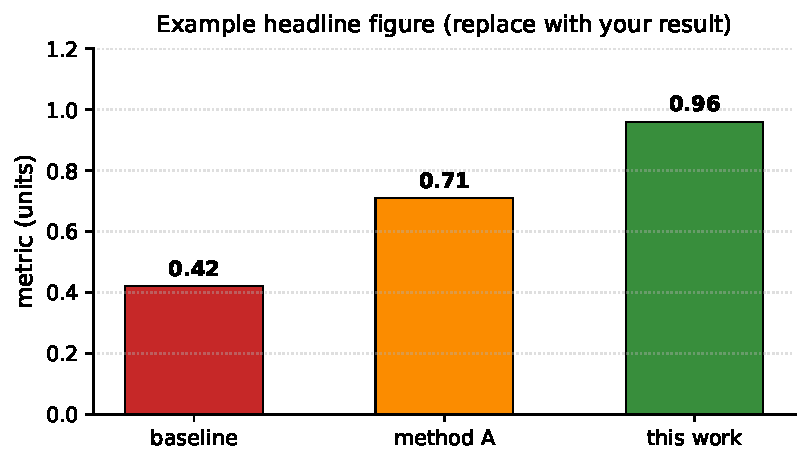
\includegraphics[width=0.62\linewidth]{figures/fig01_example.pdf}
\caption{Supplementary illustration (template-shipped figure). The
load-bearing structural figure for this paper is
Fig.~\ref{fig:structure}; this panel is retained only as a placeholder
illustration and carries no measured claim.}
\label{fig:supp}
\end{figure}

% =========================================================================
\section{Finding}
\label{sec:finding}

The three results compose into a single inversion. Read in order, they
move from a refuted intuition, to its architectural root cause, to a
constructive repair that turns the cause into an advantage:

\begin{enumerate}\itemsep0.35em
\item \textbf{Init-RNG, not learning (\tierRed).} The variability that
looked like substrate-native exploration is plain initialization
randomness. Pinning the init removes it; software reproduces the same
functional diversity with a random seed. There is no unique silicon
learning-dynamics feature to harvest. This reverses the naive ``AKIDA =
intrinsic non-determinism'' claim for this lane and config.
\item \textbf{Determinism by design (\tierGreen).} The reason is
architectural: the AKD1000 is a fully-digital 28\,nm fixed-point
event-based SNN ASIC with no stochastic primitive. It \emph{is} genuinely
neuromorphic in the dominant industry sense (event-based, sparse,
rank-order coding) --- this is \emph{not} ``fake neuromorphic'' --- but the
analog-stochastic flavor the original premise assumed is absent by design.
The Loihi contrast is decisive: a digital chip \emph{can} expose
programmable stochasticity, so Akida's determinism is a deliberate design
choice, not an inevitability of being digital.
\item \textbf{Auditable quantum non-determinism (\tierGreen).} The repair
injects ANU quantum vacuum-fluctuation entropy at exactly the init-seed
lever H\_921 located. The result is a deterministic body fed by a quantum
free-will seed, with every variation traceable to a specific ANU window.
\end{enumerate}

\paragraph{Determinism as a feature, not a limitation.} The central
inversion: because the chip is deterministic, the injected entropy enters
through a \emph{single} point and the same quantum seed always reproduces
the same output. That is precisely what makes the non-determinism
\emph{auditable} --- one provenance-traceable entry, no hidden hardware
noise to confound the trace. A chip with intrinsic analog noise could not
offer this guarantee. The AKD1000's determinism, framed as a limitation by
the original intuition, is the enabling feature of an auditable
quantum-coupled system.

\paragraph{Reconciling the falsification with the prior observations.} The
falsification does not contradict the earlier records that motivated the
intuition; it disambiguates two distinct axes that those records conflated.
The prior result that a software numpy approximation could not be made
byte-identical to the chip is a \emph{hardware-versus-software} divergence:
two different systems (a fixed-point event-based ASIC and a floating-point
numpy emulation) producing different weights, which remains valid as
``software is not byte-identical to hardware.'' The run-to-run Hamming
distances \(\{28,38,34,38\}\) are a \emph{hardware-versus-hardware}
observation under the \emph{default} (unpinned) init --- exactly condition
B of Table~\ref{tab:h921}, where the default-init RNG is free. H\_921's new
axis is hardware-versus-hardware under a \emph{pinned} init, and on that
axis the chip's learning is deterministic. The three observations are
mutually consistent once the variation is correctly attributed to
initialization rather than to learning dynamics; the apparent
``substrate non-determinism'' was a measurement that never pinned the seed.

\paragraph{Why the intuition was plausible.} The mistake was natural. The
word ``neuromorphic'' carries an analog, noisy connotation from the
biological substrate it evokes, and the literature does contain genuinely
stochastic neuromorphic systems --- analog memristor crossbars with
intrinsic device noise, and Loihi's programmable synaptic-noise primitive.
An observer who saw run-to-run variation on a chip marketed as
``brain-inspired'' had every reason to read it as physics-rooted
stochasticity. The discipline that broke the illusion was not skepticism but
\emph{control}: pinning the one variable (the seed) the naive protocol left
free. The general lesson is that a non-determinism claim about any
substrate must control its initialization before it can be attributed to
the substrate's dynamics.

% =========================================================================
\section{Verdict matrix}
\label{sec:verdicts}

\medskip
\noindent\fbox{\parbox{0.97\linewidth}{\small\textbf{Tier rubric.}
\tierBlue\ closed-form identity \(\cdot\)
\tierGreen\ numerical (reproducible probe + persisted output) \(\cdot\)
\tierYellow\ cited (DOI / arxiv / vendor / neutral profile) \(\cdot\)
\tierOrange\ install-gated / downstream-deferred \(\cdot\)
\tierRed\ falsified (kept as an honest negative, never deleted).}}

\begin{table}[h]
\centering
\small
\begin{tabular}{@{}>{\raggedright\arraybackslash}m{6.3cm} c >{\raggedright\arraybackslash}m{5.8cm}@{}}
\toprule
\textbf{Claim} & \textbf{Tier} & \textbf{Verdict pointer (verbatim stdout)} \\
\midrule
Non-det = init-RNG, not learning (pinned A=1, no-pin B>1) & \tierRed &
\texttt{.verdicts/921\_\ldots\_functional\_advantage/} \texttt{init\_seeded\_not\_learning.txt} \\
AKD1000 = digital fixed-point ASIC, det by design (5-axis) & \tierGreen &
\texttt{.verdicts/922\_\ldots\_architecture/} \texttt{digital\_deterministic\_by\_design.txt} \\
ANU quantum coupling: D1=2/16, D2=16/16, D3=TRUE & \tierGreen &
\texttt{.verdicts/923\_akida\_qrng\_coupling/anu\_seeded\_pass.txt} \\
Statistical quality ANU == chacha20 PRNG (non-claim) & \tierYellow &
\texttt{\#123-A QA6 audit (JSD 0.000433; NIST SP\,800-22 7/7)} \\
Emit-seed / R2-noise injection-point wiring & \tierOrange &
deferred (H\_923 M6; DECODER determinism invariant preserved) \\
\bottomrule
\end{tabular}
\caption{Every paper claim links to its persisted verdict. The three
terminal results are \tierRed{}/\tierGreen{}/\tierGreen{}; the honest
non-claim is cited (\tierYellow{}); the only \tierOrange{} item is an
explicit deferral, not a body claim.}
\label{tab:verdicts}
\end{table}

% =========================================================================
\section{Limitations and honest caveats}
\label{sec:limits}

\begin{itemize}\itemsep0.25em
\item \textbf{Toy scale, single chip.} All on-chip measurements use one
physical AKD1000 with a \texttt{FullyConnected} + \texttt{AkidaUnsupervised}
toy task (\texttt{units=10}, \texttt{weights\_bits=1}, \texttt{num\_weights=2},
\texttt{competition=0.1}). The H\_921 falsification is decisive for this
lane/config; it does not claim every config (larger competition,
convolutional, multi-pass) behaves identically --- a ladder would be needed
to generalize.
\item \textbf{No better-randomness claim.} The repo's \#123-A QA6 audit
finds ANU quantum bytes and a chacha20 PRNG statistically indistinguishable:
JSD \(=0.000433\) (\(23\times\) under the NIST threshold), with \(7/7\)
NIST SP\,800-22 tier-1+ tests passing~\cite{nistSP80022}. We therefore do
\emph{not} claim QRNG yields higher-quality randomness. The value claimed is
provenance (physical quantum origin), auditability, algorithmic-attack
immunity, and ontology --- not better statistics.
\item \textbf{Not a consciousness claim.} Nothing here is a
phenomenal-consciousness claim. ``Free-will seed'' is a structural label for
the init-entropy injection point, not a metaphysical assertion.
\item \textbf{Architecture scope.} H\_922 covers AKD1000 / \texttt{IpVersion.v1}
/ \texttt{NSoC\_v2}, with gen2/AKD1500-class corroboration from an FPGA cloud
session (learning disabled). A real AKD1500 silicon on-chip-learning run
would tighten this, though the architecture class (8-bit fixed point, no
noise primitive) is the same. Analog neuromorphic chips are a different
class and out of scope. Citations are corroborating mechanism; the terminal
evidence is the H\_921 measurement.
\item \textbf{Downstream wiring deferred.} The remaining injection points
(R2 spontaneous-noise and emit-seed, replacing the GPU temperature knob) and
the anima emit-pipe wiring are \tierOrange{} follow-ups; the inference
decoder's determinism is held invariant.
\end{itemize}

% =========================================================================
\section{Reproducibility}
\label{sec:repro}

Code and verdicts: \url{https://github.com/dancinlab/anima}. The three
verbatim verdicts live under \texttt{.verdicts/921\_*}, \texttt{.verdicts/922\_*},
\texttt{.verdicts/923\_*}; the probes are \texttt{PLASTICITY/h921\_nondet\_source\_probe.py},
\texttt{h923\_qrng\_seed\_probe.py}, \texttt{h923\_richtask\_probe.py}, and the
live ANU puller \texttt{mirror/qmirror/seed/anu\_pull.py}. Companion data
records: \texttt{companion/} (\texttt{verify-ledger.json},
\texttt{pr-roll.json}, \texttt{session-journal.md}). Build: \texttt{make}
(xelatex \(\times 3\) + bibtex). Page count: \texttt{make pages}.

% =========================================================================
\section{Conclusion}
\label{sec:conclusion}

Neuromorphic determinism is a design choice, not an inevitability. On the
BrainChip Akida AKD1000, the non-determinism that looked intrinsic is
init-seeded RNG (\tierRed); the root cause is a fully-digital fixed-point
ASIC with no stochastic primitive, where Loihi proves a digital chip could
have chosen otherwise (\tierGreen); and the missing non-determinism is
repaired by injecting audited ANU quantum vacuum-fluctuation entropy at the
located init lever, with the chip's determinism making that injection
single-entry and auditable (\tierGreen). The headline is not ``quantum is
better randomness'' --- it is that a deterministic neuromorphic body plus an
external, provenance-traceable quantum seed yields \emph{auditable} quantum
non-determinism, and the body's determinism is the feature that makes it so.
The single most important follow-up is the richer-task and multi-chip ladder
that turns the toy-scale repair into a production-scale entropy lane,
together with wiring the emit-seed injection point into the anima pipeline.

% =========================================================================
\paragraph{Acknowledgments.}
This work used the \texttt{hexa-lang} verification surface and the
\texttt{sidecar/paper} scaffold, the \texttt{pi5-akida} live AKD1000 host,
and the ANU Quantum Random Numbers service. LLM collaborator: Claude Opus
4.8 (1M context).

% =========================================================================
\bibliographystyle{plainnat}
\bibliography{references}

\end{document}
